\documentclass[12pt,a4paper]{article}
\usepackage[legalpaper, portrait, margin=3cm]{geometry}
\usepackage{fancyhdr}
\usepackage{amsmath}
\usepackage{amssymb}
\usepackage{graphicx}
\usepackage{blindtext}
\usepackage{hyperref}
\usepackage{indentfirst}
\usepackage{float}
\usepackage{biblatex}
\usepackage[Symbol]{upgreek}

\graphicspath{ {./} }
\hypersetup{
  colorlinks=true,
  linkcolor=blue,
  filecolor=magenta,
  urlcolor=blue,
  citecolor=blue,
  pdftitle={Relatório ASA - Projeto 1 - 2022/2023},
  pdfpagemode=FullScreen,
}
\addbibresource{./bibliography.bib}

\pagestyle{fancy}
\fancyhf{}
\rhead{Grupo \textbf{al013}}
\lhead{Relatório Projeto 1 ASA 2022/2023 LEIC-A}
\cfoot{Gonçalo Sampaio Bárias (103124)}

\renewcommand{\footrulewidth}{0.2pt}

\renewcommand{\labelitemii}{$\circ$}
\renewcommand{\labelitemiii}{$\diamond$}

\begin{document}
  \section{Descrição do Problema e da Solução}

  O problema proposto foi o de achar o número de configurações \textbf{distintas} de ladrilhar com quadrados uma área retangular, delimitada por um caminho em escada.
  O caminho em escada foi representado através de um vetor que guarda os limites máximos de cada degrau, pois representar o retângulo em forma de matriz gastaria demasiada memória e tempo.
  Assim, cada entrada do vetor contém um valor entre 0 e o comprimento máximo do retângulo.

  Esta solução teve por base uma abordagem em \textbf{programação dinâmica}.
  Neste caso, os subproblemas considerados são obtidos a partir do problema anterior subtraindo valores a uma ou mais linhas do vetor.
  O algoritmo começa sempre por remover ladrilhos da linha mais acima na coluna da direita do retângulo, isto porque é uma das maneiras que permite manter toda a informação do caminho em escada num só vetor, pois basta atualizar o valor máximo das colunas em cada linha à medida que se removem ladrilhos.
  Para se encontrar a \textbf{posição a partir da qual se remove um ladrilho}, percorre-se o vetor, começando na linha 0, até se achar a linha com maior valor.
  Caso exista mais do que uma linha com o maior valor, tomamos como posição inicial a primeira encontrada.
  Para saber o \textbf{tamanho máximo do ladrilho} que é possível inserir para a esquerda e para baixo nessa posição, basta contar quantas entradas consecutivas a partir dessa posição têm o mesmo valor.
  Quando todas as entradas do vetor estiverem a 0 o algoritmo retorna como resposta o valor 1, para indicar que aquela é uma configuração desejável.
  Para guardar os valores dos subproblemas, para que o algoritmo não os tenha de recalcular, é usada uma \textit{tabela de dispersão}.
  Quando as chamadas recursivas do algoritmo terminam, é retornado o valor para a chamada anterior, onde mapeamos na \textit{tabela de dispersão} o valor do subproblema com uma chave que representa o estado do vetor nesse momento.
  Por fim, o algoritmo retorna a soma de todos os valores retornados pelos subproblemas, apresentando assim a resposta final do problema.

  \section{Análise Teórica}

  Sendo $N$ a largura da escada.

  \begin{itemize}
    \setlength{\itemsep}{0pt}
    \item Simples leitura do input, colocando cada elemento num vetor. Logo, $\Theta(N)$.
    \item Para verificar se chegámos às respostas dos subproblemas é necessário, no pior caso, percorrer todas as entradas do vetor até acharmos uma diferente de 0. Logo, $O(N)$.
    \item Para achar a linha de onde se vai remover o próximo ladrilho, é necessário percorrer sempre todas as entradas do vetor até achar a entrada com valor máximo. Logo, $\Theta(N)$.
    \item Para achar o tamanho máximo do ladrilho que cabe numa dada posição para a esquerda e para baixo, é necessário percorrer, no pior caso, todas as entradas do vetor na situação em que a posição está na primeira linha e temos todas as entradas com valores iguais. Logo, $O(N)$.
    \item A função de dispersão utilizada percorre todos os elementos do vetor. Logo, $\Theta(N)$.
    \item A obtenção dos resultados dos subproblemas a partir da \textit{tabela de dispersão}, bem como a inserção de tais valores na \textit{tabela de dispersão} são feitas no pior caso em tempo linear. Logo, $O(N)$.
    \item A aprensentação do resultado é feita em tempo constante. Logo, $\Theta(1)$.
  \end{itemize}

  O número total de caminhos em escada possíveis num quadrado de lado n é dado pelo número de maneiras de percorrer, do canto superior esquerdo para o canto inferior direito, linhas paralelas no interior do quadrado, separadas de forma unitária.
  Deste modo, sabemos que o número total de caminhos em escada é dado por $2N \choose N$, pois só podemos percorrer tais linhas para baixo e para a direita.
  Existe uma aproximação deste resultado, \textit{Stirling's approximation}\cite{enwiki:1126871905}, que é dada por $\frac{2^{2N}}{\sqrt{N\pi}}$.
  Assim, no melhor caso, um algoritmo que pretende achar todas as maneiras de ladrilhar um quadrado teria esta complexidade temporal, pois estamos a assumir que a operação de obter um novo caminho em escada a partir de um outro seria $O(1)$.
  Na verdade como o algoritmo proposto faz essa operação em $O(n)$ e não desconstrói o quadrado em caminhos em escada só para baixo e para a direita, também faz caminhos para a esquerda, então sabemos que terá uma complexidade temporal pior, mas da mesma ordem de grandeza que a mencionada.
  Assim, a complexidade global da solução é exponencial.

  \section{Avaliação Experimental dos Resultados}

  O programa foi executado, pelo menos 10 vezes para cada caminho em escada recorrendo ao programa \href{https://github.com/sharkdp/hyperfine}{\textit{hyperfine}}.

  \begin{figure}[H]
    \centering
    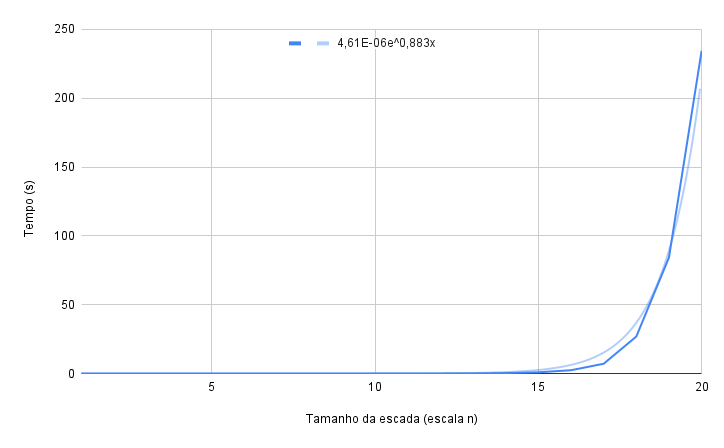
\includegraphics[width=5in]{report.png}
    \caption{Complexidade temporal do problema proposto}
    \label{fig:graphic}
  \end{figure}

  De realçar que, por uma questão de simplicidade, na análise experimental, as escadas usadas foram quadrados, ou seja, $N = M$.
  Os dados revelam uma reta exponencial, tal como concluído na análise teórica.

  \printbibliography[title={Referência}]

\end{document}
Footer
